% Created 2021-07-30 Fri 11:37
% Intended LaTeX compiler: pdflatex
\documentclass[presentation,mathserif,table]{beamer}
\usepackage[utf8]{inputenc}
\usepackage[T1]{fontenc}
\usepackage{graphicx}
\usepackage{grffile}
\usepackage{longtable}
\usepackage{wrapfig}
\usepackage{rotating}
\usepackage[normalem]{ulem}
\usepackage{amsmath}
\usepackage{textcomp}
\usepackage{amssymb}
\usepackage{capt-of}
\usepackage{hyperref}
\beamertemplatenavigationsymbolsempty
\usepackage[T1]{fontenc}
\usepackage{DejaVuSans}
\usepackage{DejaVuSansMono}
\usefonttheme{professionalfonts}
\usepackage[euler-digits,euler-hat-accent]{eulervm}
\setbeamertemplate{itemize items}{•}
\setbeamertemplate{enumerate items}[default]
\setbeamertemplate{headline}{}
\setbeamertemplate{footline}{
\leavevmode%
\hbox{%
\begin{beamercolorbox}[wd=\paperwidth,ht=2.25ex,dp=1ex,right]{fg=black}%
\usebeamerfont{section in head/foot}\insertsection\hspace*{2em}
\insertframenumber{} / \inserttotalframenumber\hspace*{2ex}
\end{beamercolorbox}%
}%
\vskip0pt%
}
\usepackage{appendixnumberbeamer}
\setbeamersize{text margin left=3mm,text margin right=3mm}
\newcommand\blfootnote[1]{%
\begingroup
\renewcommand\thefootnote{}\footnote{#1}%
\addtocounter{footnote}{-1}%
\endgroup
}
\setbeamerfont{footnote}{size=\tiny}
\usepackage{tikz}
\usepackage[retainorgcmds]{IEEEtrantools}
\hypersetup{colorlinks=true, allcolors=., urlcolor=blue}
\usepackage[absolute,overlay]{textpos}
\newcommand{\eg}{e.g.\,}
\newcommand{\ie}{i.e.\,}
\newcommand{\aka}{a.k.a.\,}
\newcommand{\etc}{\emph{etc.}\,}
\newcommand{\X}{{\mathbold X}}
\newcommand{\bS}{{\mathbold S}}
\newcommand{\bSigma}{{\mathbold \Sigma}}
\newcommand{\x}{{\mathbold x}}
\newcommand{\bbeta}{{\mathbold \beta}}
\newcommand{\Y}{{\mathbold Y}}
\newcommand{\y}{{\mathbold y}}
\newcommand{\B}{{\mathbold B}}
\newcommand{\W}{{\mathbold W}}
\newcommand{\U}{{\mathbold U}}
\newcommand{\V}{{\mathbold V}}
\newcommand{\bH}{{\mathbold H}}
\newcommand{\R}{\mathbb{R}}
\DeclareMathOperator*{\argmin}{argmin}
\DeclareMathOperator*{\argmax}{argmax}
\DeclareMathOperator*{\tv}{TV}
\DeclareMathOperator*{\Tr}{Tr}
\DeclareMathOperator*{\FFT}{FFT}
\DeclareMathOperator*{\IFFT}{IFFT}
\DeclareMathOperator*{\diag}{diag}
\DeclareMathOperator*{\supp}{supp}
\DeclareMathOperator*{\tf}{tf}
\DeclareMathOperator*{\idf}{idf}
\DeclareMathOperator*{\df}{df}
\DeclareMathOperator*{\Var}{Var}
\DeclareMathOperator*{\Frob}{Frob}
\DeclareMathOperator*{\F}{F}
\DeclareMathOperator*{\softmax}{softmax}
\DeclareMathOperator*{\AUC}{AUC}
\usepackage{bm}
\usecolortheme{dove}
\setbeamercolor*{block title example}{fg=black,bg=white}
\setbeamercolor*{block body example}{fg=black,bg=white}
\usetheme{default}
\author{Jerome Dockes}
\date{}
\title{ML Part 2 tutorial}
\author{Jérôme Dockès \& Nikhil Bhagwat}
\titlegraphic{
\includegraphics[height=1.5cm]{figures/mcgill-university.png} \hspace{1.5cm} 
\includegraphics[height=1.5cm]{figures/origami-lab-logo.png}}
\date{QLS course 2021-07-30}
\subtitle{Dimensionality reduction \& cross-validation}
\hypersetup{
 pdfauthor={Jerome Dockes},
 pdftitle={ML Part 2 tutorial},
 pdfkeywords={},
 pdfsubject={},
 pdfcreator={Emacs 26.3 (Org mode 9.3.7)}, 
 pdflang={English}}
\begin{document}

\maketitle
\begin{frame}[label={sec:org4a48b89}]{Problem setting}
\begin{equation}
Y = f(X) + E
\end{equation}
\vspace{-10pt}
\begin{itemize}
\item \(Y \in \R\): output (\aka target, dependent variable) to predict
\item \(X \in \R^p\): features (\aka inputs, regressors, descriptors, independent variables)
\item \(E \in \R\): unmodelled noise
\item \(f\): the function we try to approximate
\end{itemize}
\end{frame}
\begin{frame}[label={sec:org3ba9110},fragile]{Parameter estimation \aka model fitting}
 Minimize a sum of:
\begin{itemize}
\item the empirical risk: error on training data
\item a regularization term
\end{itemize}
\begin{block}{Example: logistic regression}
\begin{equation}
\argmin_{\bbeta, \beta_0} \frac{1}{2} \| \bbeta \|_2^2 + C \sum_{i=1}^n \log(\exp(-y_i \, (\X_i^T \, \bbeta + \beta_0)) + 1)
\end{equation}
\end{block}
\begin{structureenv} %% params
\begin{itemize}
\item \(\bbeta, \beta_0\): parameters to be \emph{estimated}
\item \(C\): hyperparameter, \emph{chosen} prior to learning
(controls amount of regularization)
\end{itemize}
\href{https://scikit-learn.org/stable/modules/generated/sklearn.linear\_model.LogisticRegression.html}{\texttt{sklearn.linear\_model.LogisticRegression}}
\end{structureenv}
\end{frame}
\begin{frame}[label={sec:orgf6f9b5e},fragile]{scikit-learn "estimator API": \texttt{fit; predict}}
 \begin{verbatim}
estimator = LogisticRegression(C=1)
estimator.fit(X_train, y_train)
predictions = estimator.predict(X_test)
\end{verbatim}
\vfill
\url{https://scikit-learn.org/stable/getting\_started.html}
\href{https://scikit-learn.org/stable/modules/generated/sklearn.linear\_model.LogisticRegression.html}{\texttt{sklearn.linear\_model.LogisticRegression}}
\end{frame}

\begin{frame}[label={sec:orgff4bd2d},fragile]{Evaluating performance with \texttt{sklearn.metrics}}
 \begin{verbatim}
estimator = LogisticRegression(C=1)
estimator.fit(X_train, y_train)
predictions = estimator.predict(X_test)

accuracy = metrics.accuracy_score(y_test, predictions)
\end{verbatim}
\vfill
\url{https://scikit-learn.org/stable/getting\_started.html}
\href{https://scikit-learn.org/stable/modules/generated/sklearn.linear\_model.LogisticRegression.html}{\texttt{sklearn.linear\_model.LogisticRegression}}
\href{https://scikit-learn.org/stable/modules/classes.html\#module-sklearn.metrics}{\texttt{sklearn.metrics}}
\href{https://scikit-learn.org/stable/modules/model\_evaluation.html\#the-scoring-parameter-defining-model-evaluation-rules}{more info on model evaluation}
\vfill
\texttt{ex\_01\_fit\_predict.py}
\end{frame}
\begin{frame}[label={sec:org981bc55},fragile]{Cross-validation}
 \begin{center}
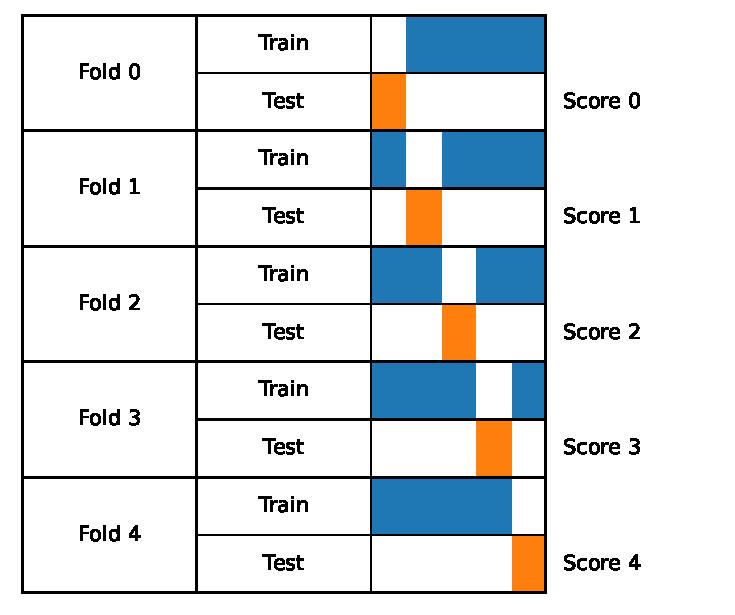
\includegraphics[height=.7 \textheight]{cv_figure_simple.pdf}
\end{center}

\href{https://scikit-learn.org/stable/modules/cross\_validation.html}{\texttt{scikit-learn.org/stable/modules/cross\_validation.html}}
\href{https://scikit-learn.org/stable/modules/generated/sklearn.model\_selection.GridSearchCV.html}{\texttt{sklearn.model\_selection.cross\_validate}}

\texttt{ex\_02\_cross\_validate.py}
\end{frame}

\begin{frame}[label={sec:org1d89a0c}]{Dataset transformations}
\begin{block}{Typical pipeline}
\begin{center}
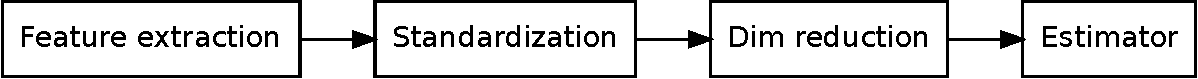
\includegraphics[width=.9\linewidth]{pipeline.pdf}
\end{center}
\end{block}

\begin{block}{Example: for autism prediction with fMRI from ML part 1}
\begin{center}
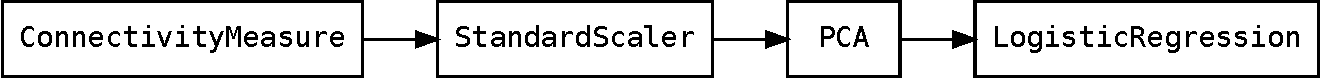
\includegraphics[width=.9\linewidth]{pipeline_example.pdf}
\end{center}
\end{block}
\end{frame}
\begin{frame}[label={sec:org9d96564},fragile]{scikit-learn "transformer API": \texttt{fit; transform}}
 \begin{verbatim}
transformer = StandardScaler()
transformer.fit(X_train)
transformed_X = transformer.transform(X_train)
\end{verbatim}
\begin{block}{can also be written:}
\begin{verbatim}
transformer = StandardScaler()
transformed_X = transformer.fit_transform(X_train)
\end{verbatim}
\end{block}
\begin{structureenv} %% links
\vfill
\href{https://scikit-learn.org/stable/modules/generated/sklearn.preprocessing.StandardScaler.html\#sklearn.preprocessing.StandardScaler}{\texttt{sklearn.preprocessing.StandardScaler}}

\href{https://scikit-learn.org/stable/getting\_started.html\#transformers-and-pre-processors}{scikit-learn "getting started"}

\href{https://scikit-learn.org/stable/data\_transforms.html}{scikit-learn "user guide"}

\vfill
\texttt{ex\_03\_transformer.py}
\end{structureenv}
\end{frame}
\begin{frame}[label={sec:org821786f},fragile]{scikit-learn "transformer API": \texttt{fit; transform}}
 \begin{verbatim}
transformer = StandardScaler()
transformed_X = transformer.fit_transform(X_train)

transformed_X_test = transformer.transform(X_test)
\end{verbatim}
\vfill
\begin{center}
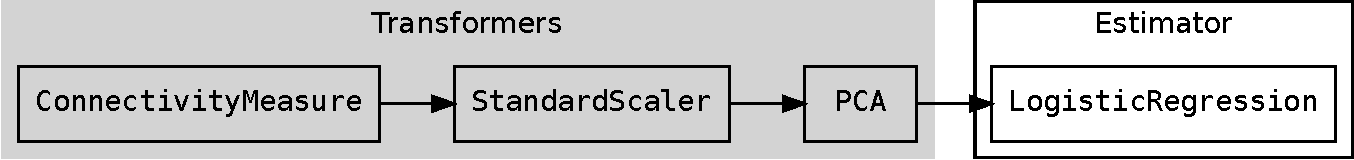
\includegraphics[width=.9\linewidth]{pipeline_transformer_estimator.pdf}
\end{center}

\href{https://scikit-learn.org/stable/modules/generated/sklearn.preprocessing.StandardScaler.html\#sklearn.preprocessing.StandardScaler}{\texttt{sklearn.preprocessing.StandardScaler}}

\href{https://scikit-learn.org/stable/getting\_started.html\#transformers-and-pre-processors}{scikit-learn "getting started"}

\href{https://scikit-learn.org/stable/data\_transforms.html}{scikit-learn "user guide"}
\end{frame}
\begin{frame}[label={sec:org02905ad},fragile]{Example: \texttt{preprocessing.StandardScaler}}
 \begin{block}{\texttt{fit:}}
Compute mean and standard deviation of each column
\end{block}
\begin{block}{\texttt{transform:}}
Subtract mean and divide by standard deviation
\end{block}
\begin{structureenv} %% link
\href{https://scikit-learn.org/stable/modules/generated/sklearn.preprocessing.StandardScaler.html\#sklearn.preprocessing.StandardScaler}{\texttt{sklearn.preprocessing.StandardScaler}}
\end{structureenv}
\end{frame}
\begin{frame}[label={sec:orgfcad261},fragile]{Example: \texttt{feature\_selection.SelectKBest}}
 \begin{block}{\texttt{fit:}}
\begin{itemize}
\item compute ANOVA or correlation for each column of \(X\)
\item Remember the indices of the \(k\) columns with highest scores
\end{itemize}
\end{block}
\begin{block}{\texttt{transform:}}
\begin{itemize}
\item Index input to keep only the \(k\) selected columns
\end{itemize}
\end{block}


\begin{structureenv} %% link
\href{https://scikit-learn.org/stable/modules/generated/sklearn.feature\_selection.SelectKBest.html\#sklearn.feature\_selection.SelectKBest}{\texttt{sklearn.feature\_selection.SelectKBest}}

\url{https://scikit-learn.org/stable/modules/feature\_selection.html}

\texttt{ex\_04\_feature\_selection.py}
\end{structureenv}
\end{frame}
\begin{frame}[label={sec:org1ed3f0a},fragile]{Example: \texttt{decomposition.PCA}}
 \begin{block}{\texttt{fit:}}
\begin{itemize}
\item Compute Singular Value Decomposition of \(\X\)
\end{itemize}
\begin{structureenv} %% Singular Value Decomposition
\begin{equation}
\X = \U \, \bS \, \V^T
\end{equation}
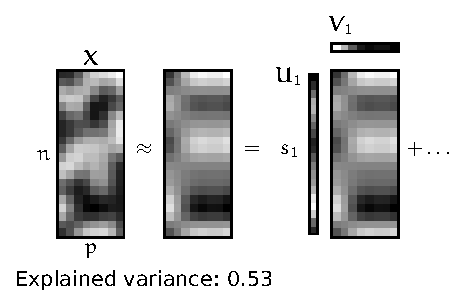
\includegraphics[height=.5 \textheight]{figures/generated/pca_step_by_step/pca_steps_1.pdf}
\end{structureenv}
\end{block}
\end{frame}

\begin{frame}[label={sec:org628d3f2},fragile]{Example: \texttt{decomposition.PCA}}
 \begin{block}{\texttt{fit:}}
\begin{itemize}
\item Compute Singular Value Decomposition of \(\X\)
\end{itemize}
\begin{structureenv} %% Singular Value Decomposition
\begin{equation}
\X = \U \, \bS \, \V^T
\end{equation}
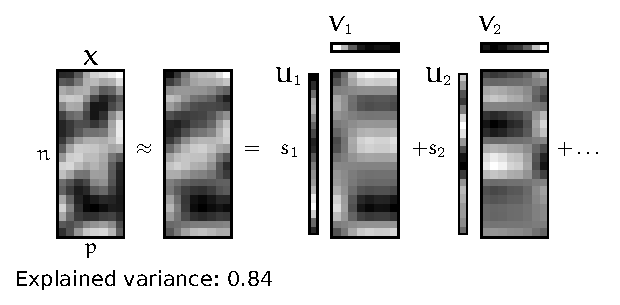
\includegraphics[height=.5 \textheight]{figures/generated/pca_step_by_step/pca_steps_2.pdf}
\end{structureenv}
\end{block}
\end{frame}

\begin{frame}[label={sec:org907b179},fragile]{Example: \texttt{decomposition.PCA}}
 \begin{block}{\texttt{fit:}}
\begin{itemize}
\item Compute Singular Value Decomposition of \(\X\)
\end{itemize}
\begin{structureenv} %% Singular Value Decomposition
\begin{equation}
\X = \U \, \bS \, \V^T
\end{equation}
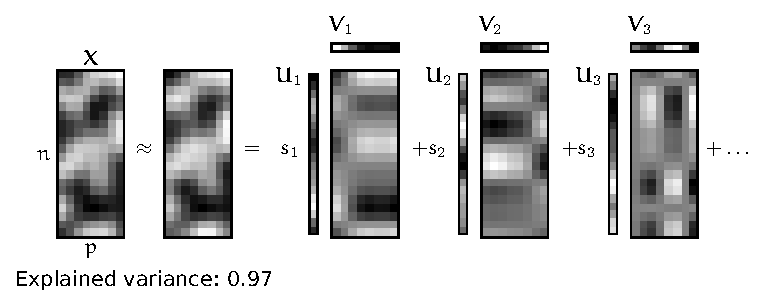
\includegraphics[height=.5 \textheight]{figures/generated/pca_step_by_step/pca_steps_3.pdf}
\end{structureenv}
\end{block}
\end{frame}

\begin{frame}[label={sec:org3c5d511},fragile]{Example: \texttt{decomposition.PCA}}
 \begin{block}{\texttt{fit:}}
\begin{itemize}
\item Compute Singular Value Decomposition of \(\X\)
\end{itemize}
\begin{equation*}
\X = \U \, \bS \, \V^T
\end{equation*}
\begin{itemize}
\item store \(\V\)
\end{itemize}
\end{block}
\begin{block}{\texttt{transform:}}
Compute projection on column space of \(\V\): simply multiply by \(\V^T\)
\begin{block}{Notes}
\begin{itemize}
\item \texttt{fit\_transform}: simply return \(\U \, \bS\)
\item \(\V^T\) is the `components\_` attribute of a fitted `PCA` instance
\end{itemize}
\end{block}
\end{block}
\begin{structureenv} %% link
\href{https://scikit-learn.org/stable/modules/generated/sklearn.decomposition.PCA.html\#sklearn.decomposition.PCA}{\texttt{sklearn.decomposition.PCA}}
\end{structureenv}
\end{frame}
\begin{frame}[label={sec:org4caf7ff},fragile]{Chaining transformations}
 Use \href{https://scikit-learn.org/stable/modules/generated/sklearn.pipeline.Pipeline.html\#sklearn.pipeline.Pipeline}{\texttt{sklearn.pipeline.Pipeline}} or \href{https://scikit-learn.org/stable/modules/generated/sklearn.pipeline.make\_pipeline.html\#sklearn.pipeline.make\_pipeline}{\texttt{sklearn.pipeline.make\_pipeline}}:
\begin{verbatim}
pipe = make_pipeline(
    standardizer, dim_reductor, estimator
)
pipe.fit(X, y)
\end{verbatim}
\begin{block}{Example:}
\begin{verbatim}
make_pipeline(
    StandardScaling(), PCA(), LogisticRegression()
)
\end{verbatim}
\end{block}
\end{frame}
\begin{frame}[label={sec:org02d6cdd}]{}
\begin{columns}
\begin{column}{.33\columnwidth}
\(\small{ \text{Var}(\hat{\beta}_i) = \mathbb{E}(\hat{\beta}_i  - \mathbb{E}(\hat{\beta}_i))^2}\)
\end{column}

\begin{column}{.38\columnwidth}
\begin{center}
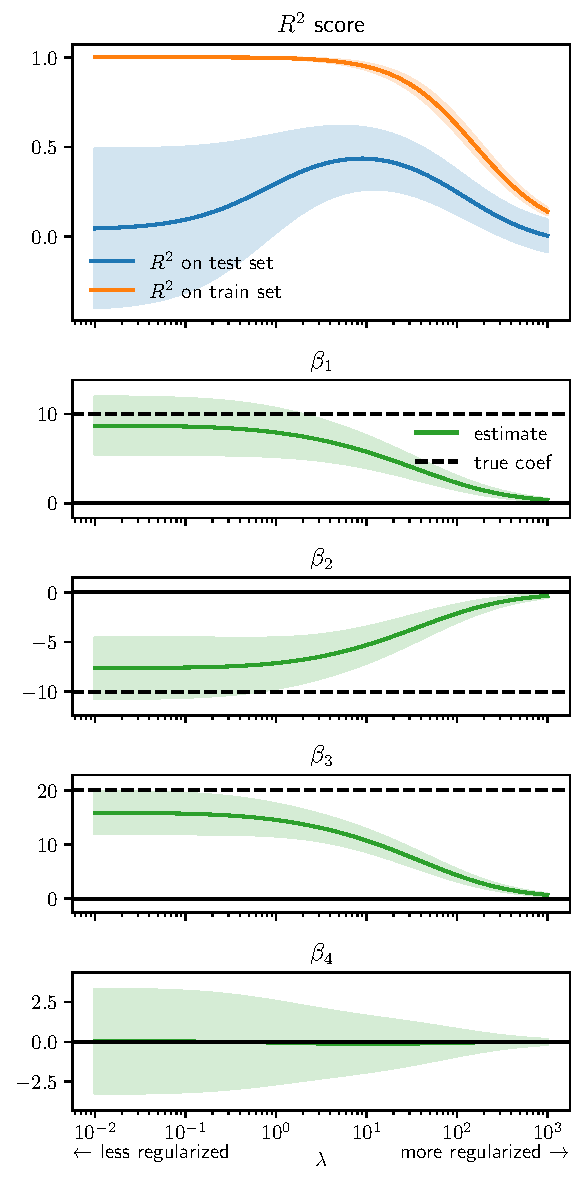
\includegraphics[height=\textheight]{ridge_regularization_path.pdf}
\end{center}
\end{column}
\begin{column}{.3\columnwidth}
\(\small \text{Bias}(\hat{\beta}_i) = \mathbb{E}(\hat{\beta}_i) - \beta_i\)
\end{column}
\end{columns}
\end{frame}
\begin{frame}[label={sec:orgf8e1d92},fragile]{Nested cross-validation}
 \begin{center}
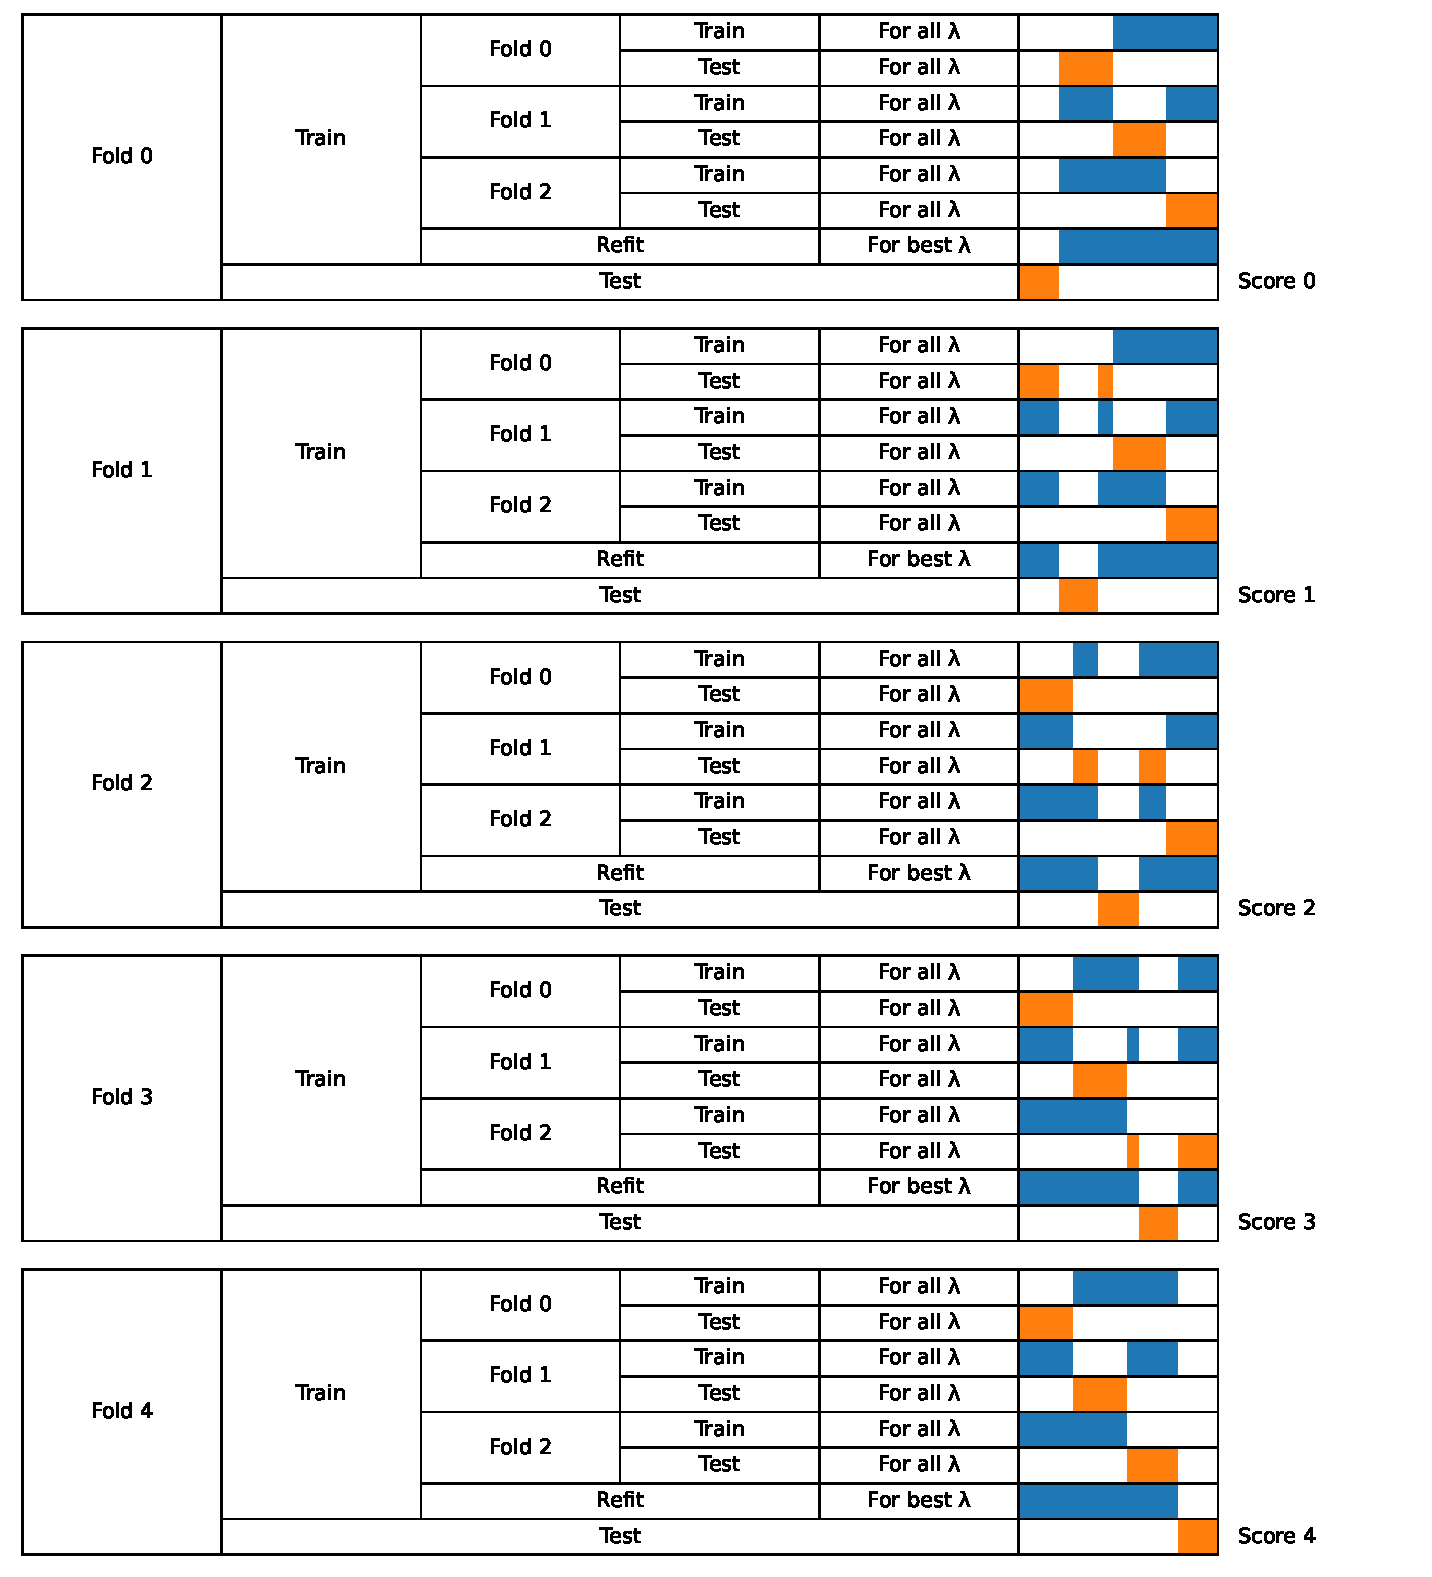
\includegraphics[width=.9\linewidth]{cv_figure_nested.pdf}
\end{center}
see  \href{https://scikit-learn.org/stable/modules/generated/sklearn.model\_selection.GridSearchCV.html}{\texttt{sklearn.model\_selection.GridSearchCV}}
\end{frame}
\begin{frame}[label={sec:org23ac710},fragile]{Implementing nested CV}
 \texttt{ex\_05\_nested\_cross\_validation.py}
\end{frame}
\begin{frame}[label={sec:orge79c59f},fragile]{Cross-validation and hyperparameter selection in scikit-learn}
 \begin{itemize}
\item \href{https://scikit-learn.org/stable/modules/classes.html\#module-sklearn.pipeline}{\texttt{sklearn.pipeline.Pipeline} or \texttt{sklearn.pipeline.make\_pipeline}}
\item \href{https://scikit-learn.org/stable/modules/generated/sklearn.model\_selection.GridSearchCV.html\#sklearn.model\_selection.GridSearchCV}{\texttt{sklearn.model\_selection.GridSearchCV}}
\item \href{https://scikit-learn.org/stable/modules/generated/sklearn.model\_selection.cross\_validate.html?highlight=cross\_validate\#sklearn.model\_selection.cross\_validate}{\texttt{sklearn.model\_selection.cross\_validate}}
\item use \texttt{*CV} estimators! \href{https://scikit-learn.org/stable/modules/generated/sklearn.linear\_model.RidgeCV.html}{\texttt{RidgeCV}}, \href{https://scikit-learn.org/stable/modules/generated/sklearn.linear\_model.LogisticRegressionCV.html}{\texttt{LogisticRegressionCV}}, \ldots{}
\end{itemize}

\begin{center}
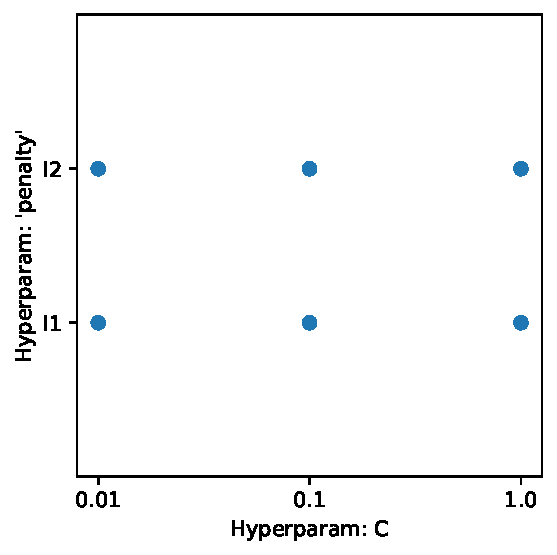
\includegraphics[height=.5 \textheight]{grid.pdf}
\end{center}
\end{frame}
\begin{frame}[label={sec:org4ed8466},fragile]{Cross-validation pitfalls}
 \begin{itemize}
\item fitting part of the pipeline on the whole data: use \texttt{Pipeline}
\item ignoring some dependencies in the data: use the appropriate \texttt{cv} iterator: \url{https://scikit-learn.org/stable/modules/cross\_validation.html\#cross-validation-iterators}
\item good cv scores on one dataset do not guarantee generalization to new data
\end{itemize}
\end{frame}
\end{document}